\documentclass{article}
\usepackage{enumerate}
\usepackage{amsmath}
\usepackage{graphicx}
\usepackage{subfigure}
\usepackage{geometry}
\def\degree{${}^{\circ}$}
\geometry{left=3.0cm,right=3.0cm,top=3.0cm,bottom=4.0cm}
\begin{document}

\section*{Problem 1.}
	$\quad \quad$When A moves upwards, if not considering the movement of B, the left row above A and below A move the same distance and the length of right row remains the origin. However, the middle row above A becomes shorter and the eliminate part moves to the lower part of B. So when A moves $x$ cm, B will move $\frac{x}{2}$ cm. Suppose the upward direction to be positive.
	\begin{enumerate}[(a)]
	\item
		\begin{eqnarray*}
			\left\{
			\begin{array}{lll}
				v_a=-2v_b\\
				v_a+v_b=24cm/s\\
			\end{array}
			\right.\quad\Rightarrow\quad
			\left\{
			\begin{array}{lll}
				v_a=16cm/s\\
				v_b=-8cm/s\\
			\end{array}
			\right.
		\end{eqnarray*}
		\begin{align*}
		a_a&=\frac{v_a}{\delta t}=2cm/s^2\\
		a_b&=\frac{v_b}{\delta t}=-1cm/s^2\\
		\end{align*}
	\item
		$$v_{bt}=a_bt=-6cm/s$$
		$$s_{bt}=\frac{1}{2}a_bt^2=-18cm$$
	\end{enumerate}
	
\section*{Problem 2.}
	$\quad \quad$Suppose the direction of $v_0$ to be the x-axis and the direction to the sky to be the y-axis, the launch point to be the zero point, then
	$$\vec{a}=-g\hat{n}_y$$
	$$\vec{v}=v_0\hat{n}_x-gt\hat{n}_y$$
	$$|\vec{a_t}|=\frac{\vec{a}\cdot\vec{v_t}}{|\vec{v_t}|}=\frac{g^2t}{\sqrt{v_0^2+g^2t^2}}$$
	$$|\vec{a_n}|=\sqrt{|\vec{a}|-|\vec{a_t}|^2}=\frac{gv_0}{\sqrt{v_0^2+g^2t^2}}$$

\section*{Problem 3.}
	$\quad \quad$Suppose the east direction to be the x-axis and the north direction to be the y-axis, the start point to be the zero point, then
	\begin{enumerate}[(a)]
	\item
		$$y=v_1t$$
		$$\vec{v}=v_1\hat{n}_x+v_2\hat{n_y}=v_1\hat{n}_x+v_0\sin\frac{v_1\pi t}{L}\hat{n_y}$$
		$$|v|=\sqrt{v_1^2+v_0^2\sin^2\frac{v_1\pi t}{L}}$$
	\item
	\item
		\begin{align*}
		s_t&=\int_0^tvdt=v_0\int_0^t\sin\frac{v_1\pi t}{L}dt\ \hat{n}_x+v_1t\ \hat{n}_y\\
		&=v_0\left[ -\frac{L}{v_1\pi}\cos \frac{v_1\pi t}{L}\right]_0^t\ \hat{n}_x+v_1t\ \hat{n}_y\\
		&=\frac{v_0L}{v_1\pi}\left( 1-\cos \frac{v_1\pi t}{L} \right)\ \hat{n}_x+v_1t\ \hat{n}_y\\
		\end{align*}
	\item
		When $t=\frac{L}{v_1}$, the canoe drifted down the river.\\
		$$s_x=\frac{v_0L}{v_1\pi}\left( 1-\cos \pi \right)=\frac{2v_0L}{v_1\pi}$$
	\end{enumerate}

\section*{Problem 4.}
	$\quad \quad$Suppose the rolling direction to be the x-axis and the direction to ground to be the y-axis, the center of the wheel to be the zero point, the origin position of P to be $(R\cos\theta_0,\ R\sin\theta_0)$, then
	\begin{enumerate}[(a)]
	\item
		$$\delta\theta=\omega\delta t$$
		\begin{eqnarray*}
			P=\left\{
			\begin{array}{lll}
				x&=R\cos (\theta_0+\omega t)+\omega Rt\\
				y&=R\sin (\theta_0+\omega t)\\
			\end{array}
			\right.(t>0)
		\end{eqnarray*}
	\item
		
	\item
		\begin{figure}[h!]
			\centering
			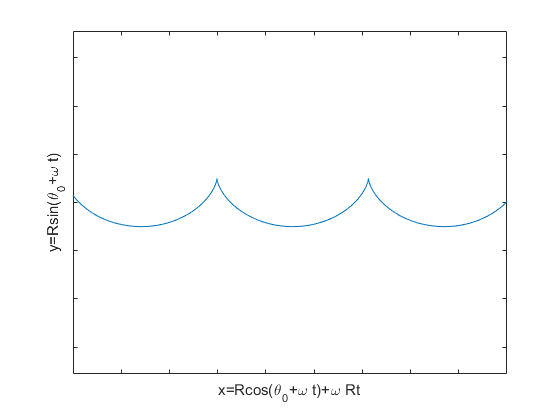
\includegraphics[width=7cm]{p4_b.png}
			\caption{trajectory of P}
			\label{fig-sample}
		\end{figure}
		
		$$\vec{v}=x'(t)\hat{n}_x+y'(t)\hat{n}_y
		=R\omega[1-\sin(\theta_0+\omega t)]\hat{n}_x
		+R\omega\cos(\theta_0+\omega t)\hat{n}_y$$
	\item
		\begin{align*}
			l&=\int_0^t\sqrt{\left(\frac{dx}{dt}\right)^2+\left(\frac{dy}{dt}\right)^2}dt\\
			&=\sqrt{2}R\omega\int_0^t\sqrt{1-\sin(\theta_0+\omega t)}dt\\
			&=\sqrt{2}R\omega\int_0^t\left|\sin\left(\frac{\theta_0+\omega t}{2}\right)-\cos\left(\frac{\theta_0+\omega t}{2}\right)\right|dt\\
			&=2R\omega\int_0^t\left|\sin\left(\frac{\omega t}{2}+\frac{2\theta_0-\pi}{4}\right)\right|dt\\
		\end{align*}
		When $t\in \left(\frac{(8k+1)\pi-2\theta_0}{2\omega},\ \frac{(8k+5)\pi-2\theta_0}{2\omega}\right)$, $\sin\left(\frac{\omega t}{2}+\frac{2\theta_0-\pi}{4}\right)>0$, $k\in R$\\
		When $t\in \left(\frac{(8k+5)\pi-2\theta_0}{2\omega},\ \frac{(8k+9)\pi-2\theta_0}{2\omega}\right)$, $\sin\left(\frac{\omega t}{2}+\frac{2\theta_0-\pi}{4}\right)<0$, $k\in R$\\
		In half of one period, i.e., $t\in\left(0,\ \frac{2\pi}{\omega}\right)$, 
		$$2R\omega\int_0^{\frac{2\pi}{\omega}}\left|\sin\left(\frac{\omega t}{2}+\frac{2\theta_0-\pi}{4}\right)\right|dt
		=4R\omega\int_0^{\frac{\pi}{\omega}}\sin\frac{\omega t}{2}dt
		=8R\left[-\cos\frac{\omega t}{2}\right]_0^{\frac{\pi}{\omega}}
		=8R$$
		\begin{eqnarray*}
			l=\left\{
			\begin{array}{lll}
				8R\left[\frac{\omega t}{2\pi}\right]+2R\omega\int_0^t\sin\left(\frac{\omega t}{2}+\frac{2\theta_0-\pi}{4}\right)dt\\
				8R\left[\frac{\omega t}{2\pi}\right]-2R\omega\int_{\frac{2\pi}{\omega}}^t\sin\left(\frac{\omega t}{2}+\frac{2\theta_0-\pi}{4}\right)dt
			\end{array}
			\right.\left.
			\begin{array}{lll}
				t\in \left[\frac{(8k+1)\pi-2\theta_0}{2\omega},\ \frac{(8k+5)\pi-2\theta_0}{2\omega}\right)\\
				t\in \left[\frac{(8k+5)\pi-2\theta_0}{2\omega},\ \frac{(8k+9)\pi-2\theta_0}{2\omega}\right)
			\end{array}
			\right.
		\end{eqnarray*}
		\begin{eqnarray*}
			l=\left\{
			\begin{array}{lll}
				4R\left\lbrace\left[\frac{\omega t}{\pi}\right]+\cos\left(\frac{2\theta_0-\pi}{4}\right)-\cos\left(\frac{\omega t}{2}+\frac{2\theta_0-\pi}{4}\right)\right\rbrace\\
				4R\left\lbrace\left[\frac{\omega t}{\pi}\right]+\cos\left(\frac{2\theta_0-\pi}{4}\right)+\cos\left(\frac{\omega t}{2}+\frac{2\theta_0-\pi}{4}\right)\right\rbrace
			\end{array}
			\right.\left.
			\begin{array}{lll}
				t\in \left[\frac{(8k+1)\pi-2\theta_0}{2\omega},\ \frac{(8k+5)\pi-2\theta_0}{2\omega}\right)\\
				t\in \left[\frac{(8k+5)\pi-2\theta_0}{2\omega},\ \frac{(8k+9)\pi-2\theta_0}{2\omega}\right)
			\end{array}
			\right.
		\end{eqnarray*}
	\end{enumerate}
	
\section*{Problem 5.}
	The unit of $c$ is $s^{-1}$ and the unit of $r_0$ is $m$. 
	\begin{enumerate}[(a)]
	\item
		$$r(t)=r_0(1-ct),\ \varphi(t)+1=\frac{1}{1-ct}$$
		$$r(t)+r(t)\varphi(t)=r_0$$
	\newpage
		\begin{figure}[h!]
			\centering
			\subfigure[$c>0$]{
			\label{Fig.sub.1}
			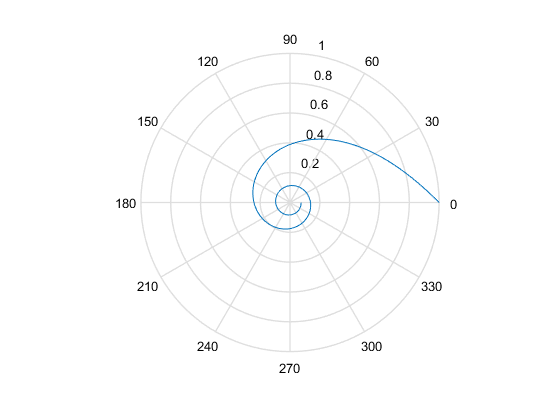
\includegraphics[width=7cm]{p5_a.png}}
			\subfigure[$c<0$]{
			\label{Fig.sub.2}
			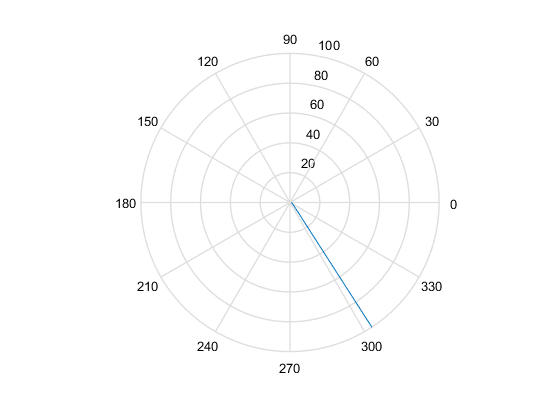
\includegraphics[width=7cm]{p5_a2.png}}
			\caption{$r(\varphi)=\frac{r_0}{\varphi+1}$}
			\label{fig-sample}
		\end{figure}
	\item
		\begin{align*}
			\vec{v_r}&=\frac{dr}{dt}\hat{n_r}=-cr_0\hat{n_r}\\
			\vec{v_\varphi}&=r\frac{d\varphi}{dt}\hat{n_\varphi}=\frac{cr_0}{1-ct}\hat{n_\varphi}\\
			|v|&=\sqrt{\vec{v_r}^2+\vec{v_\varphi}^2}=\frac{|cr_0|\sqrt{2-2ct+c^2t^2}}{1-ct}
		\end{align*}
	\item
		\begin{align*}
			\vec{a_r}&=\left[\frac{d^2r}{dt^2}-r\left(\frac{d\varphi}{dt}\right)^2\right]\hat{n_r}=-\frac{c^2r_0}{(1-ct)^3}\hat{n_r}\\
			\vec{a_\varphi}&=\left(r\frac{d^2\varphi}{dt^2}+2\frac{dr}{dt}\frac{d\varphi}{dt}\right)\hat{n_\varphi}=\left(-\frac{2c^2r_0}{(1-ct)^2}+\frac{2c^2r_0}{(1-ct)^2}\right)\hat{n_\varphi}=\vec{0}\\
		\end{align*}
	\item
		When $c>0$, $\varphi\in(-\infty,-1)\cup(0,+\infty)$, $r\in(0,r_0)$\\
		When $c<0$, $\varphi\in(-1,0)$, $r\in(r_0,+\infty)$
	\end{enumerate}
	
\section*{Problem 6.}
	$\quad \quad$Suppose right to to be the x-axis and the direction to the sky to be the y-axis, point A to be the zero point, $\theta$ to be the angle between rod AB and the x-axis, then
	\begin{enumerate}[(a)]
	\item
		$$\theta(t)=2(\varphi_0+\dot{\varphi}t)$$
		$$x=b\cos\theta,\ y=b\cos\theta$$
		$$v_x=-2\dot{\varphi}b\sin\theta,\ v_y=2\dot{\varphi}b\cos\theta$$
		$$a_x=-4\dot{\varphi}^2b\cos\theta,\ a_y=-4\dot{\varphi}^2b\sin\theta$$
		$$|\vec{a}|=\sqrt{a_x^2+a_y^2}=4\dot{\varphi}^2b$$
		So the acceleration of pin B is of constant magnitude.
	\item
		$$\vec{a}=-4\dot{\varphi}^2b\cos\theta\hat{n_x}-4\dot{\varphi}^2b\sin\theta\hat{n_y}
		=-4\dot{\varphi}^2b(\cos\theta\hat{n_x}+\sin\theta\hat{n_y})$$
		the direction of the acceleration of pin B is the direction from pin B to Point A
	\end{enumerate}

\section*{Problem 7.}
	\begin{enumerate}[(a)]
	\item
		$$\vec{v}=\frac{dr}{dt}\hat{n_r}+r\frac{d\varphi}{dt}\hat{n_\varphi}$$
		$$\tan\alpha=\frac{|\vec{v_\varphi}|}{|\vec{v_r}|}
		=\frac{\left|r\frac{d\varphi}{dt}\hat{n_\varphi}\right|}{\left|\frac{dr}{dt}\hat{n_r}\right|}
		=\frac{rd\varphi}{dr}$$
		$$\tan\alpha\frac{dr}{r}=d\varphi$$
		Do integral on both side,
		$$\tan\alpha\ lnr=\varphi+C$$
		As $\varphi(0)=0$ and $r(0)=r_0$,
		$$C=\tan\alpha\ lnr_0$$
		$$\tan\alpha\ lnr=\varphi+\tan\alpha\ lnr_0$$
		$$ln\left(\frac{r}{r_0}\right)\sin\alpha=\varphi\cos\alpha$$
	\item
		$$ln\left(\frac{r}{r_0}\right)=\frac{\varphi}{\tan\alpha}$$
		$$r(\varphi)=r_0e^{\frac{\varphi}{\tan\alpha}}$$
		$$r'(\varphi)=\frac{1}{\tan\alpha}r_0e^{\frac{\varphi}{\tan\alpha}}$$
		$$\int_0^{\varphi}\sqrt{r(\varphi)^2+r'(\varphi)^2}d\varphi
		=\frac{r_0}{\sin\alpha}\int_0^{\varphi}e^{\frac{\varphi}{\tan\alpha}}d\varphi
		=\frac{r_0}{\sin\alpha}\left(\tan\alpha e^{\frac{\varphi}{\tan\alpha}}-1\right)$$
		\begin{eqnarray*}
			l=\left\{
			\begin{array}{lll}
				\frac{r_0}{\sin\alpha}\left(\tan\alpha e^{\frac{\varphi}{\tan\alpha}}-1\right)\\
				not\ defined\\
				2\pi r_0\\
			\end{array}
			\right.\ \left.
			\begin{array}{lll}
				\alpha\in(0,\frac{\pi}{2})\cup(\frac{\pi}{2},\pi)\\
				\alpha=0\ or\ \pi\\
				\alpha=\frac{\pi}{2}\\
			\end{array}
			\right.
		\end{eqnarray*}
	\newpage	
	\item

	\item
		\begin{figure}[h!]
			\centering				
			\subfigure[$\alpha\in(0,\frac{\pi}{2})$]{
			\label{Fig.sub.1}
			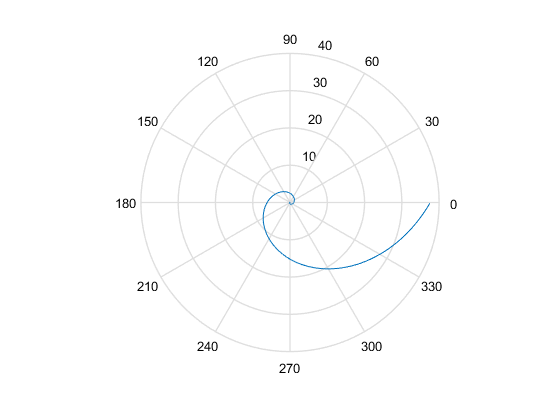
\includegraphics[width=5cm]{p7_c.png}}
			\subfigure[$\alpha=\frac{\pi}{2}$]{
			\label{Fig.sub.2}
			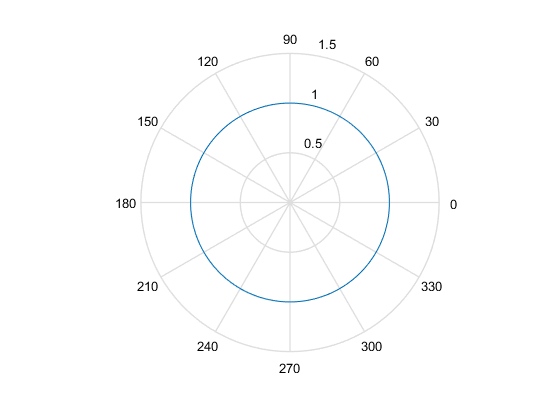
\includegraphics[width=5cm]{p7_c2.png}}
			\subfigure[$\alpha\in(\frac{\pi}{2},\pi)$]{
			\label{Fig.sub.3}
			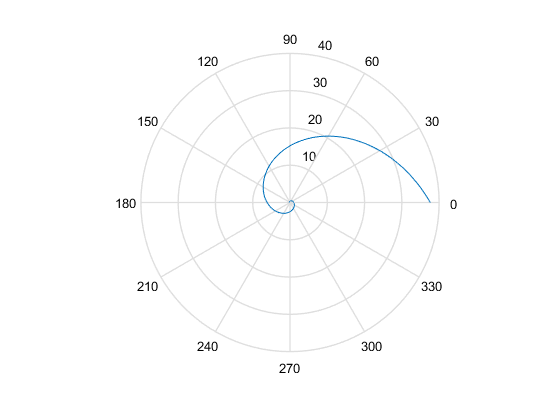
\includegraphics[width=5cm]{p7_c3.png}}
			\caption{$r(\varphi)=r_0e^{\frac{\varphi}{\tan\alpha}}$}
			\label{fig-sample}
		\end{figure}
		
		When $\alpha\in(0,\frac{\pi}{2})$, the solution is a helix as shown in Figure 3(a)\\
		When $\alpha=\frac{\pi}{2}$, the solution is a circle as shown in Figure 3(b)\\
		When $\alpha\in(\frac{\pi}{2},\pi)$, the solution is a helix as shown in Figure 3(c)\\
		When $\alpha=0$ or $\pi$, the direction of $\vec{v}$ and $\vec{r}$ are same or opposite, so the trajectory is a line but the equation and length can't be calculated because of lack of conditions.\\
		
		
	\end{enumerate}
	
\section*{Problem 8.}
	$$r=r_0-ct$$
	$$\vec{v}=\frac{dr}{dt}\hat{n_r}+r\frac{d\varphi}{dt}\hat{n_\varphi}$$
	$$v^2=c^2+r^2\left(\frac{d\varphi}{dt}\right)^2$$
	$$\frac{d\varphi}{dt}=\frac{\sqrt{v^2-c^2}}{r_0-ct}$$
	$$\frac{dt}{r_0-ct}\sqrt{v^2-c^2}=d\varphi$$
	Do integral on both side,
	$$-\frac{\sqrt{v^2-c^2}}{c}ln\left(\frac{1}{r_0-ct}\right)=\varphi+C$$
	As $\varphi(0)=0$ and $r(0)=r_0$,
	$$-\frac{\sqrt{v^2-c^2}}{c}ln\left(\frac{r}{r_0}\right)=\varphi$$
	$$r(\varphi)=r_0e^{-\frac{c\varphi}{\sqrt{v^2-c^2}}}$$
\end{document}